\documentclass[tikz, border=5mm]{standalone}
\usepackage{amsmath}
\usetikzlibrary{intersections, backgrounds, calc, patterns}

\begin{document}

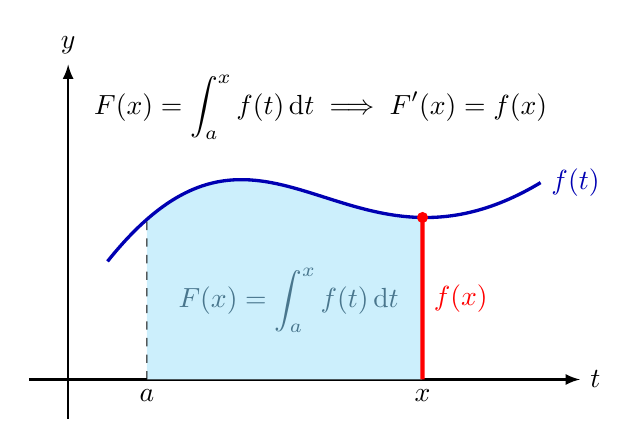
\begin{tikzpicture}[>=latex, font=\sffamily, thick]
	
	% 1. Define the Curve Path
	% We use 'name path' to find intersections later
	\path[name path=curve] (0.5, 1.5) 
	.. controls (2.5, 4.0) and (3.5, 1.0) .. (6.0, 2.5);
	
	% 2. Define coordinates for 'a' and 'x'
	\def\xa{1} % Position of a
	\def\xx{4.5} % Position of x
	
	% 3. Vertical lines paths for intersections
	\path[name path=lineA] (\xa, 0) -- (\xa, 4);
	\path[name path=lineX] (\xx, 0) -- (\xx, 4);
	
	% 4. Find Intersection Points automatically
	\path[name intersections={of=curve and lineA, by=A}];
	\path[name intersections={of=curve and lineX, by=X}];
	
	% 5. Draw Axes
	\draw[->] (-0.5, 0) -- (6.5, 0) node[right] {$t$};
	\draw[->] (0, -0.5) -- (0, 4.0) node[above] {$y$};
	
	% 6. Fill the Area (The Integral / F(x))
	\begin{scope}
		% Clip the drawing area to the rectangle between a and x
		\clip (\xa, 0) rectangle (\xx, 4);
		% Fill the area under the curve
		\fill[cyan!20] (0.5, 1.5) 
		.. controls (2.5, 4.0) and (3.5, 1.0) .. (6.0, 2.5) 
		|- (0,0) -- cycle;
	\end{scope}
	
	% 7. Draw the Curve visible on top
	\draw[blue!70!black, line width=1.2pt] (0.5, 1.5) 
	.. controls (2.5, 4.0) and (3.5, 1.0) .. (6.0, 2.5)
	node[right] {$f(t)$};
	
	% 8. Draw Dashed Lines and Labels for 'a' and 'x'
	\draw[dashed, thin] (\xa, 0) node[below] {$a$} -- (A);
	\draw[dashed, thin] (\xx, 0) node[below] {$x$} -- (X);
	
	% 9. Highlight f(x) (The Derivative)
	% We use a red line to show that the height is the rate of change
	\draw[red, line width=1.5pt] (\xx, 0) -- (X) node[midway, right] {$f(x)$};
	\fill[red] (X) circle (2pt);
	
	% 10. Label the Area F(x)
	\node[cyan!50!black] at (2.8, 1) {$\displaystyle F(x)=\int_a^xf(t)\,\mathrm{d}t$};
	
	% 11. Add the Theorem Text Box
	\node[
	anchor=north west, 
%	fill=white, 
%	draw=gray!30, 
%	rounded corners, 
%	inner sep=8pt
	] 
	at (0.2, 4) {
		$\displaystyle F(x) = \int_a^x f(t)\,\mathrm{d}t
		\implies F'(x) = f(x)$
	};
	
\end{tikzpicture}

\end{document}